\documentclass[12pt,letterpaper]{article}
\usepackage[spanish]{babel}
\usepackage[utf8]{inputenc}
\usepackage{graphicx}
\usepackage{pst-pdf}
\usepackage{amssymb}
\usepackage{hyperref}
\usepackage{listings}
\title{{Proyecto CPP2020}}
\author{Daniel Reyes Barrera}
\date{18 de diciembre de 2020}

\begin{document}
\maketitle

\abstract{En este documento se ha programado dos algoritmos para calcular la Tranformada de Fourier, la DFT (Discrete Fourier Transform) y la FFT (Fast Fourier Transform) comparando los tiempos de ejecucion para distintos $N$ n\'umeros de muestras.} 



\section{Discrete Fourier Transform}

La DFT transforma una funci\'on matem\'atica en otra, obteniendo una representaci\'on en el dominio de la frecuencia, siendo la funci\'on original una funci\'on en el dominio del tiempo.

La secuencia de $N$ n\'umeros complejos $ x_0 , ..., x_{N-1} $ se transforma en la secuencia de $N$ n\'umeros complejos $ X_0 , ..., X_{N-1} $ mediante la DFT con la f\'ormula
$$
 X(k) = \sum_{n=0}^{N-1} x(n) e ^ {- \frac{i2\pi}{N}kn} \ \ \ \ \ \ \ k = 0,..., N-1
$$

\subsection{Problema computacional.}
\textbf{Objetivo:} Calcular la transformada de fourier da una funci\'on dada.

\textbf{Entrada:} Un n\'umero entero N representando la cantidad de muestras.

\textbf{Salida:} El tiempo de ejecuci\'on de cada $N$ muestra.

\subsection{Algoritmo.}
Para el algoritmo se utiliz\'o una funci\'on de prueba $f(x) = 2sin(2 \pi x) + 5cos(2 \pi x) $ y se us\'o la libreria \texttt{complex} para manipular n\'umeros complejo. Siguiendo la formula como se define la DFT el algoritmo es sensillo de programar.

El c\'odigo fuente del programa se muestra en el ap\'endice \ref{code:DFT_1d}.
\subsection{Instancia del problema.}
Como prueba de escritorio, se seleccion\'o la siguiente instancia del problema. Entrada: $N=65536$. La salida del programa se observa en la Figura \ref{fig:DFT_1d}.
\begin{figure}[ht!]
  \centering
  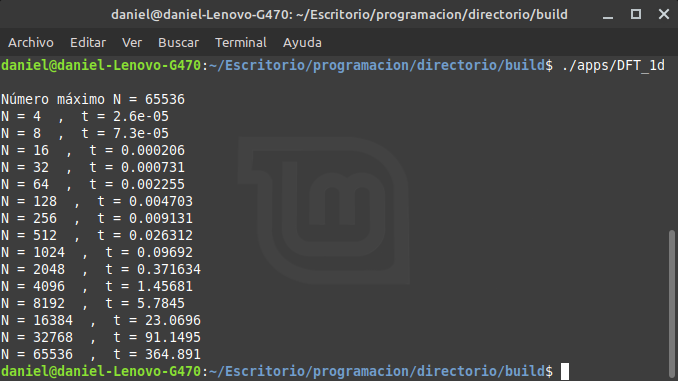
\includegraphics[width=0.8\textwidth]{figures/DFT_1d}
  \caption{Ejecución del programa.}
  \label{fig:DFT_1d}
\end{figure}
\newpage

\section{Fast Fourier Transform}

La FFT no es una nueva transformada sino que se trata de un algoritmo para el c\'alculo de la Transformada Discreta de Fourier (DFT). Su importancia radica en el hecho que elimina una gran parte de los c\'alculos repetitivos a que est\'a sometida la DFT, por lo tanto se logra un c\'alculo m\'as r\'apido. Adem\'as, la FFT generalmente permite una mayor precisi\'on en el c\'alculo de la DFT disminuyendo los errores de redondeo.

\subsection{Problema computacional.}
\textbf{Objetivo:} Calcular Transformada de fourier mediante FFT.

\textbf{Entrada:} Un n\'umero entero N representando la cantidad de muestras.

\textbf{Salida:} El tiempo de ejecuci\'on de cada $N$ muestra.

\subsection{Algoritmo.}
Al igual que el DFT se utiliz\'o la misma funci\'on de prueba y mismas librerias junto con los metodos de la clase \texttt{Complex} para la programaci\'on del algoritmo FFT.
\subsection{Instancia del problema.}
Como prueba de escritorio, se seleccion\'o la siguiente instancia del problema. Entrada: $N=33554432$, el cual es significativamente mayo que la instancia en el DFT ya que el algoritmo FFT es mucho m\'as eficiente. La salida del programa se observa en la Figura \ref{fig:DFT_1d}.
\begin{figure}[ht!]
  \centering
  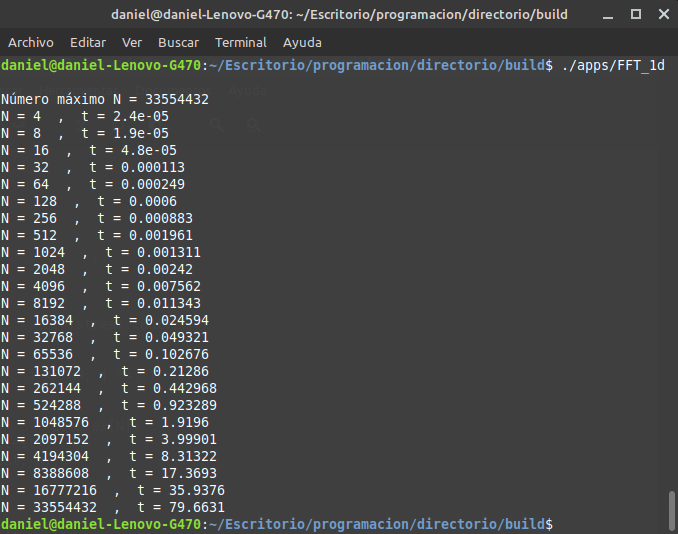
\includegraphics[width=0.8\textwidth]{figures/FFT_1d}
  \caption{Ejecución del programa.}
  \label{fig:FFT_1d}
\end{figure}

\newpage

\section{Comparaci\'on entre DFT y FFT}

Comparando los datos de tiempo de ejecuci\'on por cada $N$ muestra entre el DFT y FFT notamos una gran diferencia entre tiempos de ejecuci\'on, lo cual tiene sentido ya que el algoritmo de DFT se utiliz\'an dos ciclos \texttt{for} uno dentro de otro de tamaño de iteraci\'o $N$ y por tanto es $O(n^2)$. Por otra parte el algoritmo de FFT se programo de tal manera en el que se dividian los datos y se utilizaba la recursividad para tener una mayor eficiencia y por ello es de tipo $nlog_2(n)$. Podemos apreciar las comparaciones de los datos en la Figur \ref{fig:primero} y en la Figura \ref{fig:segundo} en distintos rangos.

\begin{figure}[ht!]
  \centering
  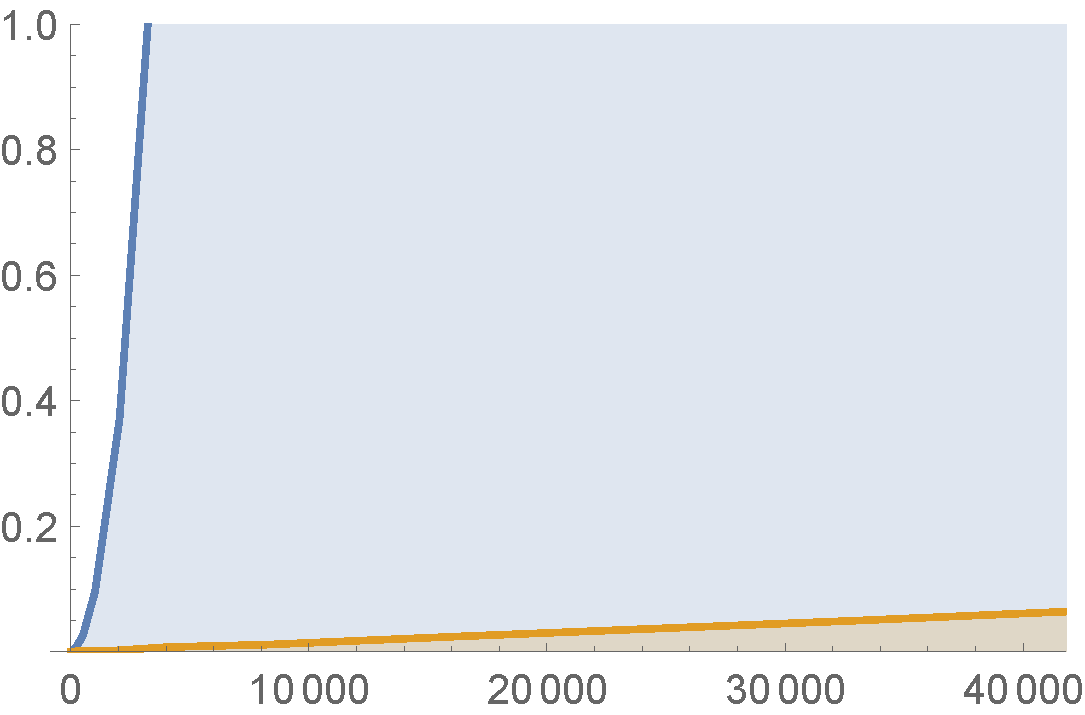
\includegraphics[width=0.8\textwidth]{figures/primero.pdf}
  \caption{Comparaci\'on de datos con un rango menor.}
  \label{fig:primero}
\end{figure}
\begin{figure}[ht!]
  \centering
  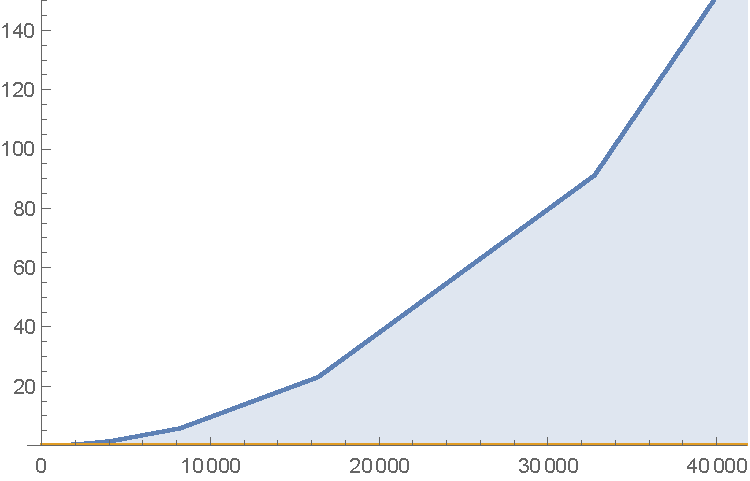
\includegraphics[width=0.8\textwidth]{figures/big.pdf}
  \caption{Comparaci\'on de datos con un rango mayor.}
  \label{fig:segundo}
\end{figure}
\begin{figure}[ht!]
  \centering
  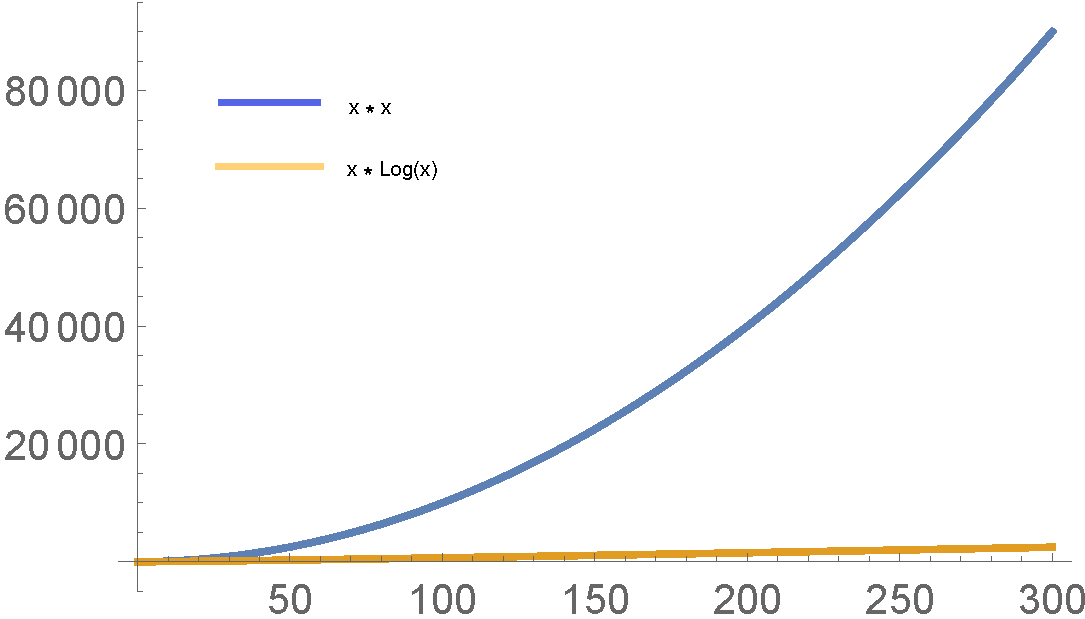
\includegraphics[width=0.8\textwidth]{figures/xx.pdf}
  \caption{Comparaci\'on entre dos funciones.}
  \label{fig:xx}
\end{figure}
\newpage


\section{Conclusiones.}
La Tramsformada Discreta de Fourier es util para el an\'alisis de señales de tiempo discreto y dominio finito pero resulta muy ineficiente al tratar con muestras grandes y por ello es indicado utilizar FFT el cual es exageradamente mas eficiente que el DFT.
La FFT es de gran importancia en una amplia variedad de aplicaciones, desde el tratamiento digital de señales y filtrado digital en general a la resoluci\'on de ecuaciones en derivadas parciales o los algoritmos de multiplicaci\'on r\'apida de grandes enteros.


\section{C\'odigo fuente de DFT} 
\label{code:DFT_1d}
\lstinputlisting[language=C++, numbers=left]{figures/DFT_1d.cpp}
\section{C\'odigo fuente de FFT} 
\label{code:FFT_1d}
\lstinputlisting[language=C++, numbers=left]{figures/FFT_1d.cpp}



\end{document}
